\documentclass{article}
\usepackage[UTF8]{ctex}
\usepackage{graphicx}
\usepackage{float} 
\usepackage{subfigure} 
\usepackage{bbding} 
\usepackage{listings}
\lstset{language=Matlab,
extendedchars=false,columns=flexible,mathescape=true}

\title{第二章作业}
\author{曾嘉翊\\16307130203}
\date{}
\begin{document}
\maketitle
\thispagestyle{empty}
1.
\begin{lstlisting}
d=linspace(0,2,101);%delta 取 0 到 2
pr(0,-1);%画出(0,-1)附近的等高线
[~,g,G] = m(0,-1);
s1=zeros(2,101);
for i=1:101
[s1(:,i),~,~,~,~]=trust(g,G,d(i));%计算 x^*
end
figure;
plot(s1(1,:),s1(2,:));%x^*  的图形
figure;%下面换成 (0,0.5) 作图
pr(0,0.5);
[~,g,G] = m(0,0.5);
s2=zeros(2,101);
for i=1:101
[s2(:,i),~,~,~,~]=trust(g,G,d(i));
end
figure;
plot(s2(1,:),s2(2,:));
function []=pr(a,b)%该函数用于画出等高线
x = linspace(a-2,a+2,201);
y = linspace(b-2,b+2,201);
[X,Y] = meshgrid(x,y);
[f,g,G] = m(a,b);
Z = f+g(1).*X+g(2).*Y+1/2*(G(1,1).*X.^2+G(2,2).*Y.^2+2*G(1,2).*X.*Y);
contour(X,Y,Z);
\end{lstlisting}


\begin{figure}[htbp]
\begin{minipage}[t]{0.6\textwidth}
\centering
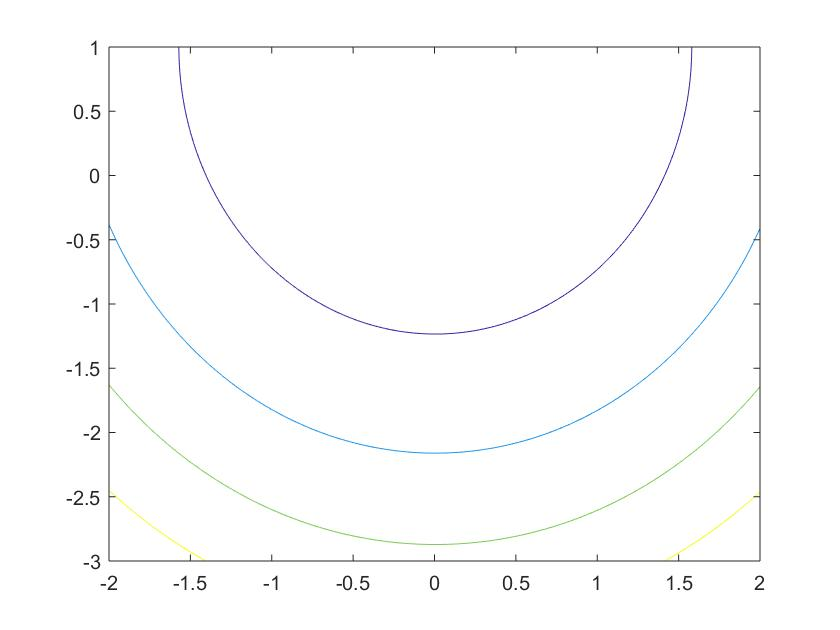
\includegraphics[width=9cm]{01g.jpg}
\caption{(0,-1)附近的等高线图}
\end{minipage}

\begin{minipage}[t]{0.6\textwidth}
\centering
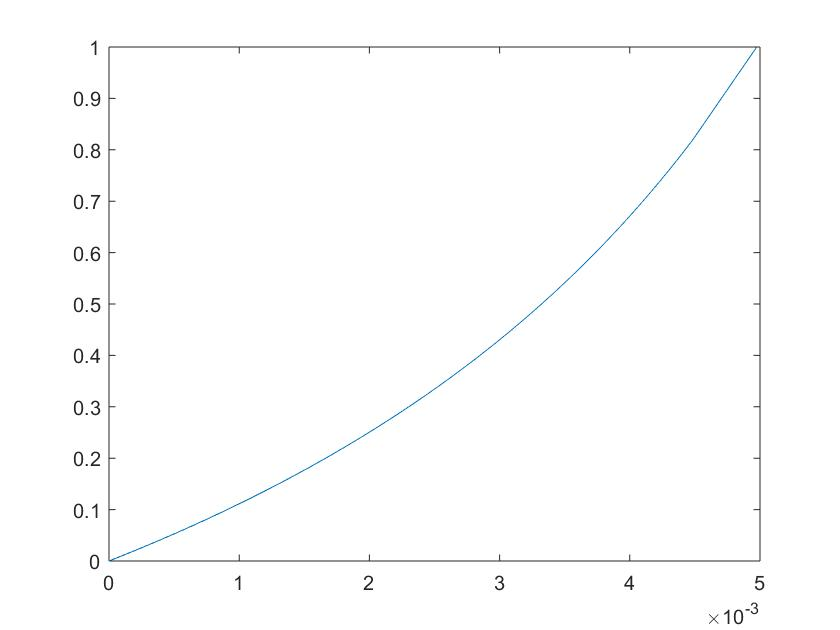
\includegraphics[width=9cm]{01x.jpg}
\caption{(0,-1)附近的$x^*$图}
\end{minipage}

\begin{minipage}[t]{0.6\textwidth}
\centering
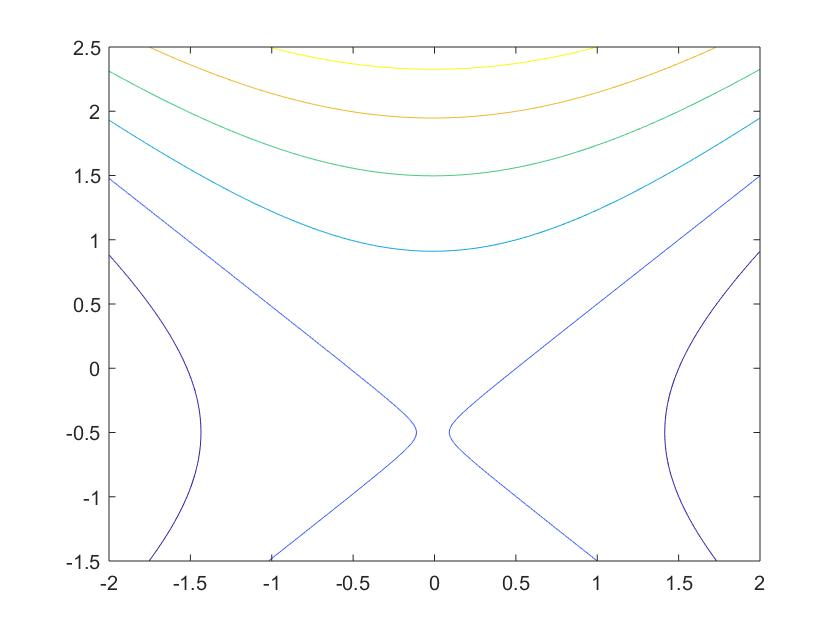
\includegraphics[width=9cm]{005g.jpg}
\caption{(0,0.5)附近的等高线图}
\end{minipage}
\end{figure}

\begin{figure}[htbp]
\begin{minipage}[t]{0.6\textwidth}
\centering
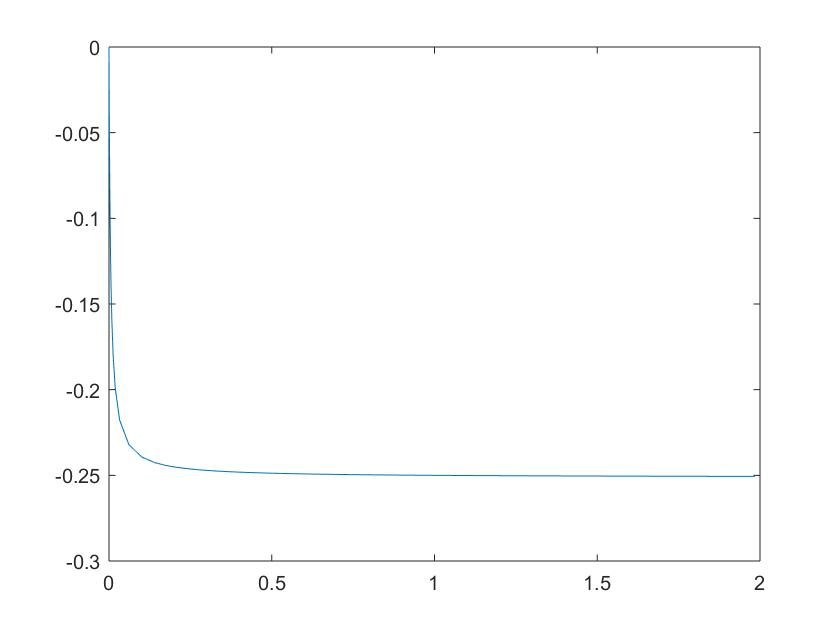
\includegraphics[width=9cm]{005x.jpg}
\caption{(0,0.5)附近的$x^*$图}
\end{minipage}
\end{figure}

\clearpage
2.
\begin{lstlisting}
deltah=1; %最大半径
x0=[2,0]'; %初始点
delta0=0.2; %初始半径
eta=0.001; %最小预测比
eps=10^(-15); %精度
i=0;%记录迭代次数
x=x0;
delta=delta0;
[~,g,G]=m(x(1),x(2));
while norm(g)>eps
    [~,g,G]=m(x(1),x(2));
    p=dogleg(g,G,delta);
    rho=(Rosenbrock(x)-Rosenbrock(x+p))/(-g'*p-1/2*p'*G*p);
    if rho<1/4
        delta=1/4*delta;
    else
        if rho>3/4 && norm(p)==delta
            delta=min(2*delta,deltah);
        end
    end
    if rho>eta
        x=x+p;
    end
    i=i+1;
end
\end{lstlisting}
输出结果为x=(1,1),迭代次数11次,用时0.017s

\clearpage
\begin{lstlisting}
deltah=1; %最大半径
x0=[2,0]'; %初始点
delta0=0.2; %初始半径
eta=0.001; %最小预测比
eps=10^(-15); %精度
i=0;%记录迭代次数
x=x0;
delta=delta0;
[~,g,G]=m(x(1),x(2));
while norm(g)>eps
    [~,g,G]=m(x(1),x(2));
    [p,~,~,~,~]=trust(g,G,delta);
    rho=(Rosenbrock(x)-Rosenbrock(x+p))/(-g'*p-1/2*p'*G*p);
    if rho<1/4
        delta=1/4*delta;
    else
        if rho>3/4 && norm(p)==delta
            delta=min(2*delta,deltah);
        end
    end
    if rho>eta
        x=x+p;
    end
    i=i+1;
end
\end{lstlisting}
输出结果为x=(1,1),迭代次数12次,用时0.041s

\end{document}